\documentclass{article}[18pt]
\ProvidesPackage{format}
%Page setup
\usepackage[utf8]{inputenc}
\usepackage[margin=0.7in]{geometry}
\usepackage{parselines} 
\usepackage[english]{babel}
\usepackage{fancyhdr}
\usepackage{titlesec}
\hyphenpenalty=10000

\pagestyle{fancy}
\fancyhf{}
\rhead{Sam Robbins}
\rfoot{Page \thepage}

%Characters
\usepackage{amsmath}
\usepackage{amssymb}
\usepackage{gensymb}
\newcommand{\R}{\mathbb{R}}

%Diagrams
\usepackage{pgfplots}
\usepackage{graphicx}
\usepackage{tabularx}
\usepackage{relsize}
\pgfplotsset{width=10cm,compat=1.9}
\usepackage{float}

%Length Setting
\titlespacing\section{0pt}{14pt plus 4pt minus 2pt}{0pt plus 2pt minus 2pt}
\newlength\tindent
\setlength{\tindent}{\parindent}
\setlength{\parindent}{0pt}
\renewcommand{\indent}{\hspace*{\tindent}}

%Programming Font
\usepackage{courier}
\usepackage{listings}
\usepackage{pxfonts}

%Lists
\usepackage{enumerate}
\usepackage{enumitem}

% Networks Macro
\usepackage{tikz}


% Commands for files converted using pandoc
\providecommand{\tightlist}{%
	\setlength{\itemsep}{0pt}\setlength{\parskip}{0pt}}
\usepackage{hyperref}

% Get nice commands for floor and ceil
\usepackage{mathtools}
\DeclarePairedDelimiter{\ceil}{\lceil}{\rceil}
\DeclarePairedDelimiter{\floor}{\lfloor}{\rfloor}

% Allow itemize to go up to 20 levels deep (just change the number if you need more you madman)
\usepackage{enumitem}
\setlistdepth{20}
\renewlist{itemize}{itemize}{20}

% initially, use dots for all levels
\setlist[itemize]{label=$\cdot$}

% customize the first 3 levels
\setlist[itemize,1]{label=\textbullet}
\setlist[itemize,2]{label=--}
\setlist[itemize,3]{label=*}

% Definition and Important Stuff
% Important stuff
\usepackage[framemethod=TikZ]{mdframed}

\newcounter{theo}[section]\setcounter{theo}{0}
\renewcommand{\thetheo}{\arabic{section}.\arabic{theo}}
\newenvironment{important}[1][]{%
	\refstepcounter{theo}%
	\ifstrempty{#1}%
	{\mdfsetup{%
			frametitle={%
				\tikz[baseline=(current bounding box.east),outer sep=0pt]
				\node[anchor=east,rectangle,fill=red!50]
				{\strut Important};}}
	}%
	{\mdfsetup{%
			frametitle={%
				\tikz[baseline=(current bounding box.east),outer sep=0pt]
				\node[anchor=east,rectangle,fill=red!50]
				{\strut Important:~#1};}}%
	}%
	\mdfsetup{innertopmargin=10pt,linecolor=red!50,%
		linewidth=2pt,topline=true,%
		frametitleaboveskip=\dimexpr-\ht\strutbox\relax
	}
	\begin{mdframed}[]\relax%
		\centering
		}{\end{mdframed}}



\newcounter{lem}[section]\setcounter{lem}{0}
\renewcommand{\thelem}{\arabic{section}.\arabic{lem}}
\newenvironment{defin}[1][]{%
	\refstepcounter{lem}%
	\ifstrempty{#1}%
	{\mdfsetup{%
			frametitle={%
				\tikz[baseline=(current bounding box.east),outer sep=0pt]
				\node[anchor=east,rectangle,fill=blue!20]
				{\strut Definition};}}
	}%
	{\mdfsetup{%
			frametitle={%
				\tikz[baseline=(current bounding box.east),outer sep=0pt]
				\node[anchor=east,rectangle,fill=blue!20]
				{\strut Definition:~#1};}}%
	}%
	\mdfsetup{innertopmargin=10pt,linecolor=blue!20,%
		linewidth=2pt,topline=true,%
		frametitleaboveskip=\dimexpr-\ht\strutbox\relax
	}
	\begin{mdframed}[]\relax%
		\centering
		}{\end{mdframed}}
\lhead{MCS - LDS}
\usepackage{qtree}

\begin{document}
\begin{center}
\underline{\huge Formal Syntax and Semantics}
\end{center}
\section{Syntax of first-order logic}
Every (well formed) formula of first order logic is constructed from \textbf{atoms} (or \textbf{atomic formula}). We completely define the \textbf{syntax} of first-order logic by defining what we mean by atoms and the constructions we are allowed to use.
\subsection{Atoms}
\begin{itemize}
\item If P is a relation symbol of arity r and $y_1,..,y_r$ are (not necessarily distinct) variables or constant symbols, then $P(y_1,...,y_r)$ is an \textbf{atom} with free variables from $y_1,...,y_r$ (this sequence can also contain constants and repeated items)
\item If C and D are constant symbols and x and y are variables then C=D, C=x and x=y are all \textbf{atoms} with, respectively, set of free variables $\varnothing, \{x\}, \{x,y\}$
\end{itemize}
The \textbf{signature} of formula is its finite set of predicate (relation) and constant symbols
\subsection{Constructions}
\begin{itemize}
\item If $\phi$ and $\psi$ are formulae, with free variables free$(\phi)$ and free$(\psi)$, then
$$\phi \vee \psi , \phi \wedge \psi , \neg \phi$$
are formulae, with, respectively, free variables $free(\phi)\cup free(\psi), free (\phi)\cup free(\psi) \ and \ free(\phi)$
\item If $\phi$ is a formula with free variables $free(\phi)$ then
$$\exists x ( \phi ) , \forall x ( \phi )$$
are formulae, both with free variables $free(\phi) \backslash \{x\}$. The occurrence of x in both formulae is a bound occurrence 
\end{itemize}
If a formula has no free variables then it is called a \textbf{sentence}
\section{Parse trees}
We can check that a formula is well formed using a parse tree (if the tree cannot be made then the formula is not well formed). We can illustrate with
$$\forall x ( \forall y ( P ( x , y ) \Leftrightarrow \neg Q ( x , y ) ) ) \wedge \exists x ( P ( C , x ) \wedge \neg Q ( x , C ) )$$
\begin{center}
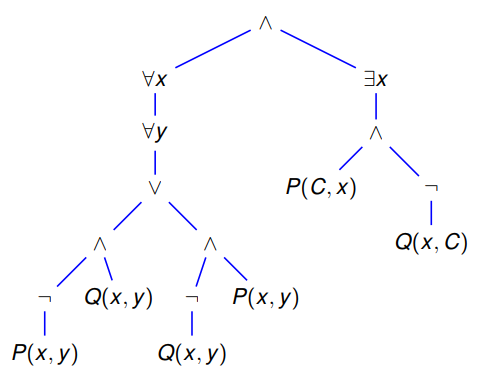
\includegraphics[scale=0.7]{tree}
\end{center}
Note that here $p\Leftrightarrow q$ has been replaced with $(p\land q)\lor (\lnot p \land \lnot q)$
\section{Semantics for first-order logic}
An interpretation or structure for a first order formula $\phi$ is:
\begin{itemize}
\item The domain of discourse D
\item A value from D for every free variables of $\phi$
\item A relation over D for every relation symbol involved in $\phi$
\item A value from D for every constant symbol involved in $\phi$
\end{itemize}
The semantics of a first order formula in some interpretation is as follows:
\begin{itemize}
\item We interpret atoms as propositional variables
\item We interpret $\land, \lor$ and $\lnot$ as propositional logic
\item We interpret $\forall x \phi$ as true if $\phi$ is true for all values for x
\item We interpret $\exists x \phi$ as true if there is at least one value for x making $\phi$ true
\end{itemize}
\section{An illustration}
Consider a \textbf{signature} consisting of two binary relation symbols P and Q and one constant symbol C. Let $\phi$ be defined as:
$$\forall x ( \forall y ( P ( x , y ) \Leftrightarrow \neg Q ( x , y ) ) ) \wedge \exists x ( P ( C , x ) \wedge \neg Q ( x , C ) )$$
In order to decide whether $\phi$ evaluates to true or not we need an \textbf{interpretation}\\
Consider the interpretation:
$$\phi = \forall x ( \forall y ( P ( x , y ) \Leftrightarrow \neg Q ( x , y ) ) ) \wedge \exists x ( P ( C , x ) \wedge \neg Q ( x , C ) )$$
where:
\begin{itemize}
\item The domain of discourse is the set of natural numbers $\mathbb{N}$
\item The relation $P = \{ ( u , v ) : u , v \in \mathbb { N } , u \leq v \}$
\item The relation $Q = \{ ( u , v ) : u , v \in \mathbb { N } , u > v \}$
\item The constant $C=0\in \mathbb{ N }$
\end{itemize}
So
\begin{itemize}
\item $(\mathbb{ N },p,Q,0)\models \phi$ if and only if\\
$( \mathbb { N } , P , Q , 0 ) \models \forall x \forall y ( P ( x , y ) \Leftrightarrow \neg Q ( x , y ) )$ and $( \mathbb { N } , P , Q , 0 ) \models \exists x ( P ( C , x ) \wedge \neg Q ( x , C ) )$
\item if and only if for every $x,y \in \mathbb{ N }, x\leqslant y \Leftrightarrow x\ngtr$ y and there exists $x\in \mathbb{ N }$ such that $0\leqslant x$ and $x\ngtr 0$
\end{itemize}
Both conjuncts are true. Thus $(\mathbb{ N },P,Q,0)$ is a model of $\phi$, i.e., $(\mathbb{ N },P,Q,0)\models \phi$
\subsection{Secondary interpretation}
Now consider a \textbf{signature} consisting of two binary relation symbols P and Q and one constant symbol C. Let $\phi$ be defined as:
$$\forall x ( \forall y ( P ( x , y ) \Leftrightarrow \neg Q ( x , y ) ) ) \wedge \exists x ( P ( C , x ) \wedge \neg Q ( x , C ) )$$
In order to decide whether $\phi$ evaluates to true or not we need an \textbf{interpretation}\\
Consider the interpretation:
$$\phi = \forall x ( \forall y ( P ( x , y ) \Leftrightarrow \neg Q ( x , y ) ) ) \wedge \exists x ( P ( C , x ) \wedge \neg Q ( x , C ) )$$
where:
\begin{itemize}
\item The domain of discourse is the set of natural numbers $\mathbb{N}$
\item The relation $P = \{ ( u , v ) : u , v \in \mathbb { N } , \textcolor{red}{u < v} \}$
\item The relation $Q = \{ ( u , v ) : u , v \in \mathbb { N } , u > v \}$
\item The constant $C=0\in \mathbb{ N }$
\end{itemize}
So
\begin{itemize}
\item $(\mathbb{ N },p,Q,0)\models \phi$ if and only if\\
$( \mathbb { N } , P , Q , 0 ) \models \forall x \forall y ( P ( x , y ) \Leftrightarrow \neg Q ( x , y ) )$ and $( \mathbb { N } , P , Q , 0 ) \models \exists x ( P ( C , x ) \wedge \neg Q ( x , C ) )$
\item if and only if for every $x,y \in \mathbb{ N }, x< y \Leftrightarrow x\ngtr$ y and there exists $x\in \mathbb{ N }$ such that $0< x$ and $x\ngtr 0$
\end{itemize}
Both conjuncts are false. Thus $(\mathbb{ N },P,Q,0)$ is not a model of $\phi$, i.e., $(\mathbb{ N },P,Q,0)\models \lnot\phi$
\section{A subtlety}
Consider a signature consisting of two binary relation symbols P and Q and one constant symbol C. Let $\phi$ be defined as
$$\forall \textcolor{blue}{x} ( \forall y ( P ( \textcolor{blue}{x} , y ) \Leftrightarrow \neg Q ( \textcolor{blue}{x} , y ) ) ) \wedge \exists z ( P ( z , \textcolor{red}{x} ) \wedge \neg Q ( \textcolor{red}{x} , C ) )$$
This is a perfectly legal formula of first order logic, even though the variable x appears "differently" in the formula
\begin{itemize}
\item x appears \textcolor{blue}{bound} in the first conjunct
\item x appears \textcolor{blue}{free} in the second conjunct
\end{itemize} 
Consequently, it is more precise to speak of "free occurrences" or "bound occurrences" of variables rather than free or bound variables
\section{Another subtlety}
Consider the formula $\chi$ defined as
$$\forall x ( \forall y ( P ( x , y ) \Leftrightarrow \neg Q ( x , y ) ) ) \wedge \exists y ( P ( y , x ) \wedge \neg Q ( x , y ) )$$
and the interpretation I for $\chi$ where:
\begin{itemize}
\item The domain D=$\{1,2,3\}$
\item $P = \{ ( 1,3 ) , ( 2,3 ) , ( 3,1 ) \}$ and $Q = \{ ( 1,1 ) , ( 1,2 ) , ( 2,1 ) , ( 2,2 ) , ( 3,2 ) , ( 3,3 ) \}$
\item x=3
\end{itemize}
Not only does x appear both free and bound but y appears bound but within the scopes of two different quantifications.\\
We clearly have $I\models \chi$ as
\begin{itemize}
\item For every $(x,y)\in D\times D, (x,y)\in P$ if and only if $(x,y)\not\in Q$
\item There exists a $y\in D$ such that $(y,3)\in P$ and $(3,y)\not\in Q$, namely y=1 (only need to show it for one value in this case as $\exists$)
\end{itemize}
If we amend the interpretation so that x is interpreted as x=2 then we have that $I\models \lnot \chi$
\section{More illustrations}
Consider the well formed formula $\phi$ defined as $\forall x \exists y P(x,y)$\\
And consider the interpretation of $\phi$ where:
\begin{itemize}
\item The domain of discourse is the set $\mathbb{Z}$ of integers
\item $P = \{ ( u , v ) : u , v \in \mathbb { Z } , u > v \}$
\end{itemize}
So,
\begin{itemize}
\item $( \mathbb { Z } , P ) = \forall x \exists y P ( x , y )$\\
if and only if for every $x \in \mathbb { Z } , ( \mathbb { Z } , P ) \models \exists y P ( x , y )$\\
if and only if for every $x\in \mathbb{ Z }$, there exists $y\in \mathbb{ Z }$ with $x>y$
\end{itemize}
For any $x\in \mathbb{ Z }$, if we take $y=x-1$ then this value of y \textbf{witnesses} that $x>y$; hence, $(\mathbb{ Z },P)\models \phi$\\
If we restrict the domain to the natural numbers $\mathbb{ N }$ and where $P = \{ ( u , v ) : u , v \in \mathbb { N } , u > v \}$, i.e. we have the restriction of $(\mathbb{ Z },p)$ to $\mathbb{ N }$ then $(\mathbb{ N },p)\models \lnot \phi$. This fails for example when a value is 0 as there is not a natural number smaller than it\\
\\
\\
Consider the well formed formula $\phi$ defined as $\exists y \forall x P ( x , y )$\\
And consider the interpretation of $\phi$ where
\begin{itemize}
\item The domain of discourse if the set $\mathbb{ Z }$ of integers
\item $P = \{ ( u , v ) : u , v \in \mathbb { Z } , u > v \}$
\end{itemize}
So,
\begin{itemize}
\item $( \mathbb { Z } , P ) = \exists y \forall x P ( x , y )$\\
if and only if there exists $y\in \mathbb{ Z }$ such that $(\mathbb{ Z },P)\models \forall x P(x,y)$\\
if and only if there exists $y\in \mathbb{ Z }$ such that for all $x\in \mathbb{ Z }, x>y$
\end{itemize}
No matter which $y\in \mathbb{ Z }$ we choose, putting $x=y-1$ results in $x\leqslant y$\\
Hence $( \mathbb { Z } , P ) \models \neg \exists y \forall x P ( x , y )$
\begin{center}{\Large
Take care with the \textbf{order} of quantifiers}
\end{center}
\end{document}